\section{Visão geral da arquitetura}

\newcommand{\frontend}{\emph{front-end}\xspace}
\newcommand{\backend} {\emph{back-end}\xspace}

A arquitetura da computação em nuvem é dividida geralmente em duas 
seções~\cite{rao-cloud-computing}, conectadas por meio de uma rede (geralmente a 
Internet):

\newcommand{\itemm}[1]{\item\textbf{#1}}

\begin{itemise}
    
    \itemm{Front-End:} É o lado visível ao cliente/usuário. Inclui o sistema ou rede
    de computador do cliente que é usada para acessar a rede. A interface é diferente
    dependendo do sistema de computação em nuvem (e-mail, etc.).

    \itemm{Back-End:} O lado usado pelo serviço oferecido, seria "a nuvem em si". 
    Inclui vários servidores, computadores, sistemas para armazenar dados, máquinas 
    virtuais... Juntas, elas constituem os serviços da computação em nuvem. O 
    \backend possui algumas responsabilidades para cumprir: implementar mecanismos 
    de segurança e controle de tráfego, e conectar computadores na rede para 
    comunicação através de protocolos (regras fixas e bem definidas).

\end{itemise}

\undef\itemm

\begin{figure}[ht]
    \centering
    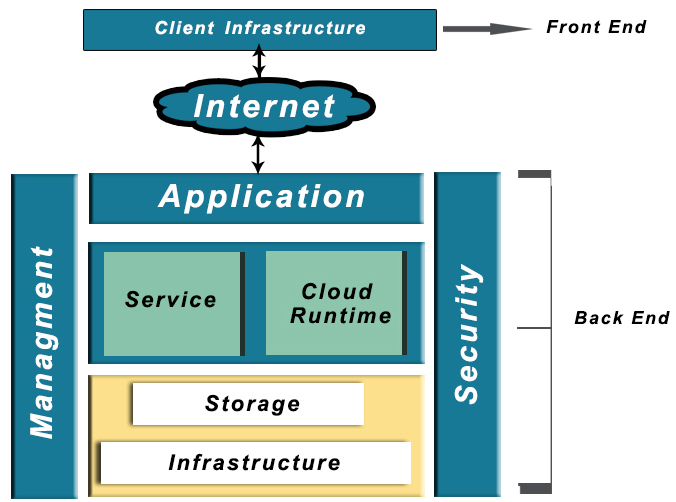
\includegraphics[width=0.5\textwidth]{img/frontBackEnd.jpg}
    \caption{Imagem retratando as duas seções principais da
        arquitetura~\cite{hostdepartment-overview-cloud}
    }
\end{figure}
